\documentclass[../main.tex]{subfiles}
\begin{document}

\begin{definition}\label{def:4.5.1}
    对 $k=1,2,\cdots$,称 $\mathrm E((X-c)^k)$ 为 $X$ 关于 $c$ 点的 \emph{$k$ 阶矩}。特别地,$c=0$ 的情况下称为 \emph{$k$ 阶原点矩},$c=\mathrm E(X)$ 的情况下称为 \emph{$k$ 阶中心矩}。
\end{definition}

根据定义可知,$\mathrm E(X)$ 为 $1$ 阶原点矩,而 $1$ 阶中心矩恒等于 $0$;$\mathrm{Var}(X)=\mathrm E(X^2)-\mathrm E^2(X)$ 为 $2$ 阶中心矩。

若 $\mathrm E(X)=\mu,\mathrm{SD}(X)=\sigma$,我们称 $\mathrm E((\frac{X-\mu}\sigma)^k)=\frac{\mathrm E((X-\mu)^k)}{\sigma^k}$ 为 \emph{$k$ 阶标准矩}。

$1$ 阶标准矩恒等于 $0$,$2$ 阶标准矩恒等于 $1$,$3$ 阶标准矩称为 $X$ 的\emph{偏度系数},记作 $\mathrm{Skew}(X)$。

\begin{example}
    $X\sim N(0,1)$,则 $\mathrm{Skew}(X)=\int_{-\infty}^{+\infty}x^3f(x)\mathrm dx=0$,其中 $f$ 为 $X$ 的 PDF。
\end{example}

我们称偏度系数 $<0$ 的分布为“负偏”或“左偏”,如图~\ref{fig:4.5.1}。

\begin{figure}[!ht]
    \centering
    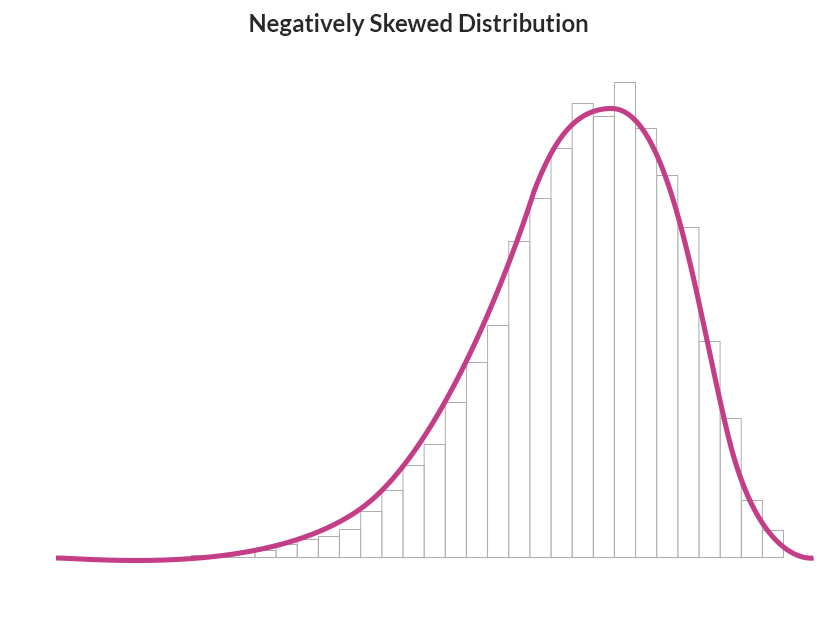
\includegraphics[scale=0.2]{figures/negative_skew.png}
    \caption{负偏分布}
    \label{fig:4.5.1}
\end{figure}

$5$ 阶以上的奇数阶标准矩计算更复杂,受噪声影响更大。

$4$ 阶标准矩称为 $X$ 的\emph{峰度系数},记作 $\mathrm{Kurt}(X)$。由于正态分布的峰度系数恒等于 $3$,因此常定义\emph{超额峰度系数}为 $\mathrm{Kurt}(X)-3$。

我们经常将 $\mu\pm\sigma$ 以内的范围称为“峰”,范围在“峰”以外但在 $\mu\pm2\sigma$ 以内的范围称为“肩”,范围在“肩”以外的部分称为“尾”。

通常,峰度系数 $>3$ 表现为相对于正态分布“尖峰厚尾”,如图~\ref{fig:4.5.2}。

\begin{figure}[!h]
    \centering
    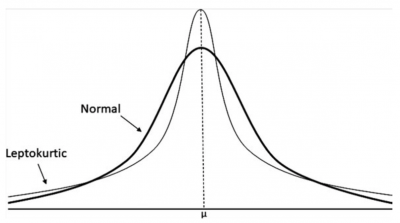
\includegraphics[scale=0.6]{figures/Leptokurtic-vs-Normal.png}
    \caption{“Leptokurtic”一词的含义即峰度系数 $>3$}
    \label{fig:4.5.2}
\end{figure}

\end{document}
